\documentclass[11pt]{article}


%----------------------------------------------------------------------------------------
%	Packages and configuration
%----------------------------------------------------------------------------------------

\usepackage[T1]{fontenc}
\usepackage{ucs}
\usepackage[francais]{babel}
\usepackage{xltxtra}
\usepackage{graphicx}
\usepackage{fontspec}
\usepackage{url}
\usepackage{float}
\usepackage[ocgcolorlinks]{hyperref}
\usepackage{fancyhdr}
\usepackage{metalogo}
\usepackage[titletoc]{appendix}
\usepackage{pdflscape} % Pour des pages au format paysage
\usepackage{enumitem}  % Pour pouvoir choisir le symbole de itemize : 
                       % \begin{itemize}[label={$\bullet$}]
\usepackage{tabu}


%\usepackage{lastpage}
\usepackage[left=3.5cm,right=3.5cm,top=2cm,bottom=2cm]{geometry}

\hypersetup{colorlinks=true,allcolors=black}

\setmainfont{Sorts Mill Goudy}
\pagenumbering{arabic}
\urlstyle{same}
%----------------------------------------------------------------------------------------
%	Header
%----------------------------------------------------------------------------------------

\newcommand{\helv}{%
   \fontsize{9}{11}\selectfont}

   \lhead{\helv \parbox[b]{3.5cm}{ÉTS - Département de génie logiciel et des TI}}
   \chead{\helv \parbox[b]{7cm}{\centering LOG792 - Proposition - Optimisation des paramètres d’une éolienne en mouvement}}
\rhead{\helv \today \\ \thepage}
\lfoot{}
\cfoot{}
\rfoot{}
\renewcommand{\headrulewidth}{0.4pt}
%\renewcommand{\footrulewidth}{0.4pt}

%----------------------------------------------------------------------------------------
%	Document
%----------------------------------------------------------------------------------------

\begin{document}

\pagestyle{fancy}

\begin{titlepage}
\thispagestyle{fancy}

\newcommand{\HRule}{\rule{\linewidth}{0.5mm}} % Defines a new command for the horizontal lines, change thickness here

\center % Center everything on the page
 
%----------------------------------------------------------------------------------------
%	HEADING SECTIONS
%----------------------------------------------------------------------------------------

\textsc{\LARGE École de Technologie Supérieure}\\[1.5cm] % Name of your university/college

\vfill

\textsc{\Large Proposition}\\[0.5cm] % Major heading such as course name
\textsc{\large Projet de fin d'études \\ Département de génie logiciel et des TI}\\[0.5cm] % Minor heading such as course title

%----------------------------------------------------------------------------------------
%	TITLE SECTION
%----------------------------------------------------------------------------------------


\HRule \\[0.4cm]
{ \huge \bfseries Optimisation des paramètres d’une éolienne en mouvement}\\[0.4cm] % Title of your document
\HRule \\[1.5cm]
 
%----------------------------------------------------------------------------------------
%	AUTHOR SECTION
%----------------------------------------------------------------------------------------
\vfill

\begin{minipage}{0.4\textwidth}
\begin{flushleft} \large
\emph{Auteur:}\\
Pierre-Alexandre \textsc{St-Jean}\\
\small{<pa@stjean.me>}
\end{flushleft}
\end{minipage}
~
\begin{minipage}{0.4\textwidth}
\begin{flushright} \large
\emph{Superviseur:} \\
Dr. Christian \textsc{Desrosiers}\\
\small{<christian.desrosiers@etsmtl.ca>}
\end{flushright}
\end{minipage}\\[4cm]

% If you don't want a supervisor, uncomment the two lines below and remove the section above
%\Large \emph{Author:}\\
%John \textsc{Smith}\\[3cm] % Your name

%----------------------------------------------------------------------------------------
%	DATE SECTION
%----------------------------------------------------------------------------------------

\vfill

{\large \today}\\[3cm] % Date, change the \today to a set date if you want to be precise

%----------------------------------------------------------------------------------------
%	LOGO SECTION
%----------------------------------------------------------------------------------------

%\includegraphics{Logo}\\[1cm] % Include a department/university logo - this will require the graphicx package
 

\end{titlepage}

%----------------------------------------------------------------------------------------
%	DOCUMENT
%----------------------------------------------------------------------------------------

\vspace*{\fill}
\begin{center}
\section*{Résumé}
\addcontentsline{toc}{section}{Résumé}
\end{center}

Le club étudiant Chinook, afin de continuer son succès en compétition améliore constament son éolienne. L'ajout d'un système mécanique et électronique de contrôle de l'angle d'attaque de celle-ci ainsi que du ratio de transmission permettron d'augmenter les performances du véhicule. Afin de commander ces nouveaux systèmes, un algorithme de contrôle doit être développé afin de géré ces systèmes. Le présent projet propose donc de caractériser l'éolienne puis de créer un tel algorithme de contrôle de l'éolienne à l'aide des algorithmes génétiques.

\vspace*{\fill}
\clearpage


\section*{Table des matières}
\addcontentsline{toc}{section}{Table des matières}

\renewcommand{\contentsname}{Table des matières}
\makeatletter
\renewcommand{\tableofcontents}{\@starttoc{toc}%
}
\makeatother

\tableofcontents

\phantomsection

\listoffigures
\addcontentsline{toc}{section}{Table des figures}


\clearpage

\section{Problématique et contexte}

Le véhicule éolien Chinook\ref{fig:chinookHall} de l'ÉTS est un regroupement de personnes\footnote{\url{http://chinookets.com}} qui analyse, conçoivent et construisent un véhicule propulsée par une éolienne. Le véhicule participe, chaque année, depuis deux ans à une compétition de véhicules de ce type qu'ils ont remportés l'année dernière. Cette année le véhicule doit être améliorer afin de pouvoir rester compétitif. Pour ce faire un système électronique de controle de l'angle d'attaque des pales de l'éolienne sera installé. La transmission du véhicule sera aussi modifiée afin de pouvoir être contrôllée électroniquement. 

\begin{figure}[H]
  \centering
  \includegraphics[width=0.5\textwidth]{images/chinook_1_et_2.jpg}
  \caption[Chinook 1 et 2]{Le Chinook 1 et le Chinook 2 en exposition dans le Hall A de l'ÉTS}
  \label{fig:chinookHall}
\end{figure}

Afin de pouvoir controller ces systèmes électroniques, des modèles de contrôle et d'optimisation de la puissance de l'éolienne doivent être créés. Les modèles théoriques applicables aux éoliennes standards doivent être modifiés afin de prendre en compte le fait que l'éolienne du Chinook est une éolienne mobile. Ainsi les systèmes de contrôles d'éoliennes fixes ne sont pas applicables dans le contexte d'une éolienne mobile.

\section{Objectifs du projet}

Le présent projet à pour but d'ammener l'éolienne du Chinook 3 [figure: \ref{fig:matRotor}] à opérer dans les conditions et à l'aide des paramètres d'opérations optimales. Pour ce faire, l'éolienne doit être caractérisé, un modèle de contrôle et d'optimisation de l'angle d'attaque ($\beta$) des pales et du ratio de transmission qui affecte la vitesse de rotation de l'éolienne ($\omega$) doit être conçu, analysé puis ce modèle doit être implanté dans le logiciel de la carte électronique de calcul.

Le système de contrôle pourra, à tout moment, changer l'angle d'attaque des pales ($\beta$) où le ratio transmission afin d'atteindre les performances optimales de l'éolienne dans les conditions de vitesse du véhicule et de vitesse du vent.


\begin{figure}[H]
  \centering
  \includegraphics[width=0.5\textwidth]{images/matetrotorrotationnel.jpg}
  \caption[Mat et Rotor du Chinook 3]{Rendu 3D du mat et du rotor du Chinook 3}
  \label{fig:matRotor}
\end{figure}

Un tel modèle ainsi opérationnel dans les systèmes de contrôle du Chinook permettra au véhicule d'atteindre de meilleures vitesses et ce plus rapidement tout en permettant de conserver les vitesses atteintes et de mieux résister aux turbulences que par les années passées.

\section{Méthodologie}

La méthode utilisé dans ce projet sera adapté à partir de plusieurs méthode d'optimisation par algorithme génétique, entre autres celles provennant de \cite{GeneticField} et de \cite{Ouissam12}. Ces méthodes seront appliqués selon des processus de génie logiciel (développement dirigé par les spécifications, etc...)

Premièrement, le facteur de conversion de l'éolienne ($C_p$) doit être caractérisé. Pour ce faire on doit récupérer des données expérimentales de l'éolienne selon plusieurs paramètres puis on doit trouver une équation qui régit ces données. Afin de trouver l'équation, une régression de style "Curve-Fitting" tel que décrite dans \cite{GeneticField} à la section 12.2 sera utilisée.

Lorsque le comportement de l'éolienne sera caractérisé, un modèle mathématique de contrôle de l'éolienne sera généré à l'aide d'un algorithme génétique. La méthode décrite dans \cite{Ouissam12} sera améliorée et adaptée afin de convenir au contexte d'utilisation du Chinook et cette méthode sera utilisée afin de générer le modèle mathématique de contrôle.

Suite à la création de la formule de contrôle et à partir de l'architecture électrique et logiciel [Annexe \ref{fig:archELE}] du Chinook 3, on peut inclure ces équations à l'intérieur du Chinook dans la carte électronique de calcul [figure \ref{fig:carteElec}]. Les équations donneront en sortie: l'angle d'attaque et le ratio de transmission à appliquer. Ces données seront envoyés aux systèmes qui contrôlent les moteurs.

\begin{figure}[H]
  \centering
  \includegraphics[width=0.7\textwidth]{images/3d-top-annoté.pdf}
  \caption[Carte électronique de calcul]{Carte électronique d'acquisition de données, de surveillance du courant électrique et de calcul de l'angle d'attaque des pales et du ratio de transmission}
  \label{fig:carteElec}
\end{figure}

Des tests sur route seront ensuite effectué avec le Chinook afin de valider si les modèles calculés à partir d'algorithmes génétiques fonctionnent.

Afin de permettre à l'éolienne de se comporter correctement lorsqu'elle est dans un autre état qu'en régime permanent, des états supplémentaires seront ajoutés à l'algorithme de contrôle, par exemple: lorsque la voiture va plus vite que l'éolienne (poussée) ou lorsqu'elle est à l'arrêt.


En résumé, le projet consiste en :
\begin{itemize}
  \item La récolte de données sur l'éolienne à différent $\beta$ et $\lambda$;
  \item La caractérisation du facteur de conversion de puissance de l'éolienne ($C_p$), c'est à dire le ratio entre la puissance du vent fournie à l'éolienne et la puissance de sortie de celle-ci;
  \item L'adaptation et l'amélioration de la méthode de \cite{Ouissam12} afin qu'elle convienne au contexte du Chinook. Cette méthode génere un modèle mathématique de contrôle de l'éolienne;
  \item l'implémentation du modèle mathématique de contrôle de l'éolienne dans la carte électronique de calcul;
  \item Les tests sur route afin de valider la méthode.
\end{itemize}

\section{Livrables et planification}
\subsection{Description des atéfacts}

\textcolor{red}{À compléter}.

\begin{itemize}[label={$\bullet$}]
  \item Projet:
  \begin{itemize}
    \item Proposition de projet
    \item Rapport d'étape
    \item Rapport final
    \item Présentation
    \item Article (description de la nouvelle méthode)
    \item Spécifications
  \end{itemize}
  \item Éolienne:
  \begin{itemize}
    \item Données de banc-d'essais
    \item Algorithme génétique de caractérisation
    \item Caractérisation de l'éolienne, $C_p$ en fonction de $\beta$ et $\lambda$
  \end{itemize}
  \item Optimisation du contrôle de l'éolienne:
  \begin{itemize}
    \item Outils de simulation
    \item Algorithme génétique d'optimisation
    \item Modèle mathématique d'optimisation de l'éolienne en fonction des caractéristiques environnantes
  \end{itemize}
  \item Carte électronique:
  \begin{itemize}
    \item implémentation de base
    \item implémentation avec modèle mathématique
  \end{itemize}
\end{itemize}

\begin{tabu} to \linewidth {X[1,l]X[2,l]}
  \bfseries Artéfact & Description \\ \hline
  Proposition de projet & Le présent document...\\
  Rapport d'étape \\
  Rapport final \\
  Présentation \\
  Article & Article scientifique décrivant la méthode utilisée pour caractériser l'éolienne et créer l'algorithme d'optimisation\\
  Spécifications \\
  \hline
  Carte électronique: implémentation de base & Implémentation permettant de faire fonctionner tout les composantes de la carte électronique et prêt à accueillir la fonction de calcul. Cet implémentation permet de faire fonctionner les modules de communication soit le XBEE, le module CAN et le module de USB-SERIAL. L'implémentation permettra aussi de faire fonctionner le module de mémoire morte (EEPROM), le module de surveillance électrique et le module d'horloge (realtime clock).\\
  Carte électronique: ajout modèle mathématique & Implémentation du modèle d'optimisation de l'éolienne à l'intérieur de la carte électronique\\

\end{tabu}
\subsection{Planification}


\textcolor{red}{À compléter}.

\begin{tabu} to \linewidth {Xlll}
  \bfseries Tâche & Début - Fin & Effort\\ \hline
  Fiche de renseignement & 26 Mars 2013 & 1h \\
  Proposition de projet  & 6 Mai 2013 - 12 Mai 2013 & 10h \\
  Rapport Final          & & \\
  Présentation           & & \\
  Article                & & \\
  Planification du projet & & \\
  \hline
  Rencontre avec professeur superviseur & (Au besoin) & \\
  \hline
  Mise en place de l'environnement de développement & & \\
  Spécification du projet & & \\
  \hline
  Programme de caractérisation de l'éolienne & & \\
  Récolte de données                         & & \\
  Caractérisation de l'éolienne              & & \\
  \hline
  Outils de simulation                   & & \\
  Programme génétique d'optimisation    & & \\
  \hline
  Carte électronique: implémentation de base    & & \\
  Carte électronique: ajout modèle mathématique & & \\
  \hline
  Tests sur route & & \\
  \hline
\end{tabu}

\section{Risques}

\textcolor{red}{À compléter}.

\begin{itemize}
  \item La complexité du projet
  \item Le manque de données
  \item Le non fonctionnement de la méthode d'optimisation
  \item Le risque que la préparation du véhicule ne respecte pas les délais
\end{itemize}



\section{Techniques et Outils}

\textcolor{red}{À compléter}.

Les spécifications logiciel et du projet seront écrites à l'aide la de la méthode (Specification by example)... \textcolor{red}{citer le livre ici}.

Formattage des documents de remise à l'aide des logiciels libres \LaTeX et de \XeLaTeX et des nombreux paquetages disponibles (CTAN\footnote{\url{http://www.ctan.org/}}).

Tout les documents et codes sources seront gérés avec le système de gestion de versions GIT\footnote{\url{http://git-scm.org}}.

Le service de partage de fichiers Dropbox sera utiliser afin de partager plusieurs fichers entre différents postes et différentes personnes.

\bibliographystyle{plainnat}
\bibliographystyle{development}
\bibliography{bibliography}
\addcontentsline{toc}{section}{Références}

\clearpage

%----------------------------------------------------------------------------------------
%	Annexes
%----------------------------------------------------------------------------------------
\section*{Annexes}
\addcontentsline{toc}{section}{Annexes}
\begin{appendices}


\section{Architecture Électrique du Chinook 3}
\label{fig:archELE}
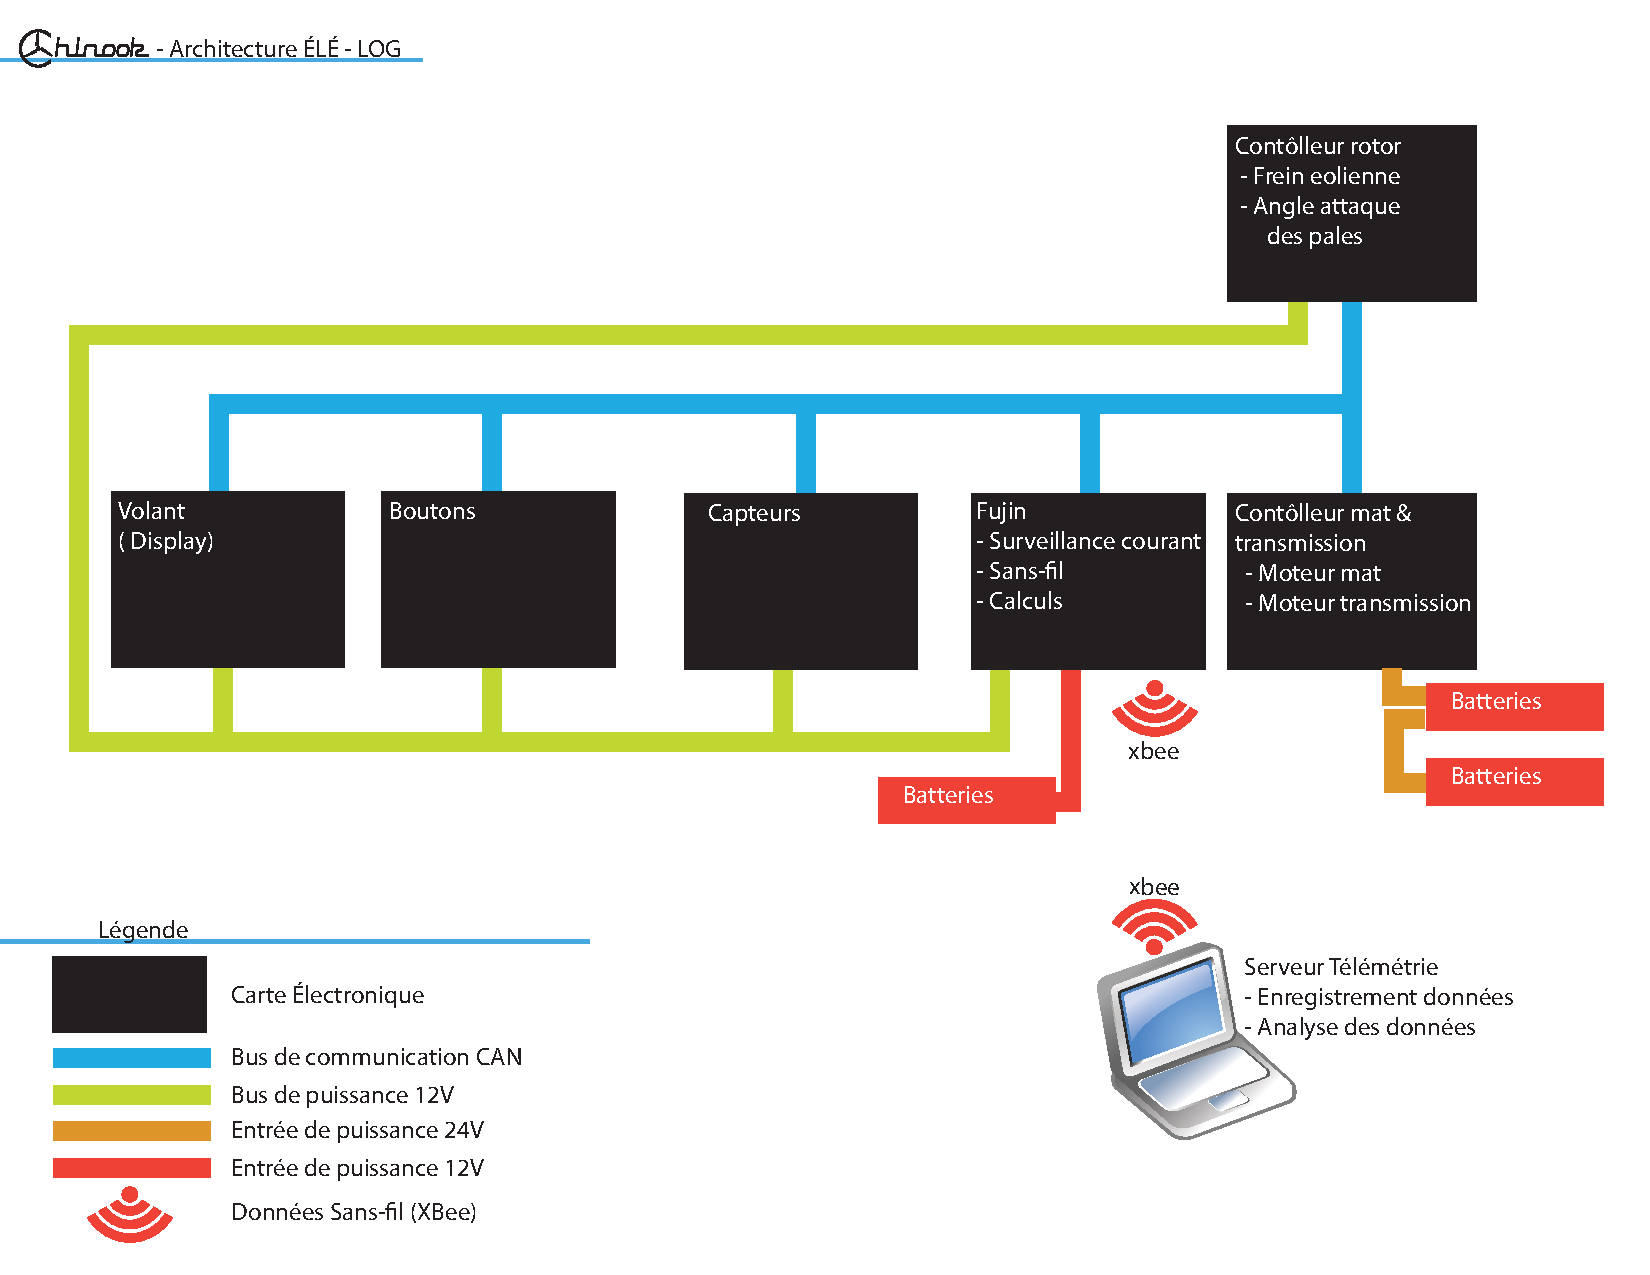
\includegraphics[height=1\textwidth,angle=90]{images/Architecture_ÉLÉ-LOG.pdf}

\end{appendices}

\end{document}
